\documentclass[12pt,a4paper]{article}
\usepackage[utf8]{inputenc}
\usepackage[T1]{fontenc}
\usepackage{amsmath, float}
\usepackage{amsfonts}
\usepackage{amssymb}
\usepackage{graphicx}
\newtheorem{lemma}{Lemma}
\newtheorem{proof}{Proof}
\usepackage{rotating}
\usepackage[colorlinks=true,linkcolor=blue, citecolor=blue, allcolors=blue ]{hyperref}

\usepackage{pgf,tikz,pgfplots}
\pgfplotsset{compat=1.15}
\usepackage{mathrsfs}
\usetikzlibrary{arrows}
\pagestyle{empty}
\newcommand{\degre}{\ensuremath{^\circ}}

\definecolor{qqwuqq}{rgb}{0,0.39215686274509803,0}
\definecolor{xdxdff}{rgb}{0.49019607843137253,0.49019607843137253,1}
\definecolor{ududff}{rgb}{0.30196078431372547,0.30196078431372547,1}

\usepackage{enumerate}

% \usepackage[left=1.00cm, right=1.00cm, top=1.00cm, bottom=1.00cm]{geometry}
\usepackage[margin=2cm]{geometry}
\author{Written by: Dick Jessen William, Reviewed by: Yip Jung Hon}
\title{MA1102R -- Calculus \\ AY2019/20 SEM 2 Solutions}

\begin{document}
	
	\maketitle
	
	\section*{Question 1}
	
	\begin{enumerate}[a.]
	    \item \begin{enumerate}[i.]
	     \item Note that $f(-1)<0$ and $f(2)>0$, hence by IVT, there is a root between $-1$ and $2$.
	    \item First, note that $f'(x) = 3x^2-2x+1 = (3x+1)(x-1)$. Also, $f(\frac{-1}{3})$ and $f(1)$ is larger than 0. This means the interval $[-\frac{1}{3},1]$ and $[1,\infty)$ have no zeroes. Since we have at most one zeroes in $(-\infty,-\frac{1}{3}]$, $f$ have at most one zeroes.
	    \end{enumerate}
	    \item
	    \begin{enumerate}[i.]
	    \item Suppose there exists two different real numbers $x,y$ so that $g(x)=g(y)$. Then,
	    \begin{align*}
	    &\frac{\sqrt{x}}{\sqrt{x}-3} = \frac{\sqrt{y}}{\sqrt{y}-3} \\
	     &\iff \sqrt{xy}-3\sqrt{x} = \sqrt{xy}-3\sqrt{y} \\
	     &\iff x = y
	    \end{align*}
	    a contradiction. Hence, $g$ is one to one.
	    \item Let $y = \frac{\sqrt{x}}{\sqrt{x}-3}$. Then, $y-1 = \frac{3}{\sqrt{x}-3}$. Hence, $\sqrt{x}-3 = \frac{3}{y-1}$ and $x = \left( 3+\frac{3}{y-1} \right)^2$. We conclude that $g^{-1}(x) = \left( 3+\frac{3}{x-1} \right)^2$
	    \item The domain of $g^{-1}$ is $\mathbb{R} \backslash \{ 1 \}$. The range is $\mathbb{R}_{\geq 0 }$
	    \end{enumerate} 
	    \item We use chain rule. Let $u = x$, $du=dx$, $dv = \sec^2{x} dx$ and $v = \tan{x}$. Then, $$\int x \sec^2{x} dx = x(\tan{x}) -\int \tan{x} dx = x\tan{x}-\ln{|\cos{x}|} +C.$$
	\end{enumerate}
	\section*{Question 2}
	\begin{enumerate}[a.]
	    \item First, recall that the 
	   $\lim_{x \rightarrow 0} \left( \frac{\sin{x}}{x} \right) = 1 $. By L-Hopital's rule,
	    \begin{align*}
	   \lim_{x \rightarrow 0} \left( \frac{1}{\sin^2{x}}-\frac{1}{x^2} \right) &= \lim_{x \rightarrow 0} \left( \frac{x^2-\sin^2{x}}{x^2 \sin^2{x}} \right) \\
	   &= \lim_{x \rightarrow 0} \left( \frac{x^2-\sin^2{x}}{x^2 \frac{\sin^2{x}}{x^2}} \right) \\
	   &= \lim_{x \rightarrow 0} \left( \frac{x^2-\sin^2{x}}{x^4} \right) \\
	   &=\lim_{x \rightarrow 0} \left( \frac{x+\sin{x}}{x} \right) \lim_{x \rightarrow 0} \left( \frac{x-\sin{x}}{x^3} \right) \\
	   &= 2\lim_{x \rightarrow 0} \left( \frac{1-cos{x}}{3x^2} \right) \\
	   &= \frac{2}{3} \lim_{x \rightarrow 0} \left( \frac{\sin{x}}{2x} \right) \\
	   &= \frac{1}{3}.
	   %There's a simpler proof online that uses sinx/x=1 https://www.quora.com/What-is-the-value-of-lim-1-sinx-2-1-x-2-when-x-0 % I see, will change the proof to the easier
	    \end{align*}
	    \item Let $\epsilon$ be given. Pick $\delta = \min\{1,\frac{2\epsilon}{7}\}$. Then, since $|x-1| < 1$, $0<x<2$. Hence, $1+x^2>1$ and $2x^2-x+1 < 7$ (This can be verified by graphing). Now, 
	    \begin{align*}
	        \left | x+\frac{1}{x^2+1}-\frac{3}{2} \right | &= \left | \frac{2x^3-3x^2+2x-1}{2(x^2+1)} \right| \\ 
	        &= \lvert \frac{(x-1)(2x^2-x+1)}{2(x^2+1)}\rvert \\
	        &< \frac{4\epsilon}{7} \frac{7}{2 \times 1} = \epsilon.
	    \end{align*}
	    Hence, the limit is $\frac{3}{2}$.
	\end{enumerate}
	% I think here it's 1+x^2 > 1, instead of >2. 
    % 	 Also think you bound for 2x^2-x+1 is wrong. Should be |x-1|<1 --> 0<x<2 --> 0<2x^2<8 --> 2x^2-x+1<9 1+x^2>1 correct, 2(2^2)-2+1 = 7 tho
	
	
    \section*{Problem 3}
    % I think this question presented clearly enough, mind if I redo it? Are you approximating sinx = x? fine by me
    \begin{enumerate}[a.]
    
    \item Note that $\sin{x} = \sin(\pi-x)$. Hence, $f(0) = f(\pi)$ by symmetry. We will find $f(0)$.
    \begin{align*}
    \lim_{x \to 0^+} \sin(x)^{\sin(x)} &= \exp\left[\lim_{x \to 0^+} \sin(x) (\ln \sin(x))\right] \\ 
    &= \exp \left[\lim_{x \to 0^+} \frac{\ln(\sin(x))}{\frac{1}{\sin(x)}}\right]
    \intertext{The top goes to $-\infty$ while the bottom goes to $\infty$. We may use L'Hopital.}
    &= \exp\left[\lim_{x \to 0^+} \frac{\frac{\cos(x)}{\sin(x)}}{-\frac{1}{\sin^2(x)}}\right]\\
    &= \exp\left[\lim_{x \to 0^+} -\frac{\sin(x)\cos(x)}{1}\right]\\
    &=1
    \end{align*}
    Hence, $f(0)= f(\pi) = 1$.
    
    \item We find the derivative of $y = \sin{x}^{\sin{x}}$. 
    Note that \begin{align*}
        y &= \sin{x}^{\sin{x}} \\
        \ln{y} &= \sin{x} (\ln{\sin{x}}) \\
        \frac{1}{y} dy &= (\cos{x} \ln{\sin{x}}+ \sin{x}\left( \frac{1}{\sin{x}} \right) \cos{x}) dx \\
        \frac{dy}{dx} &= y(\cos{x} \ln{\sin{x}}+\cos{x}) \\
        &= \sin{x}^{\sin{x}} (\cos{x} \ln{\sin{x}}+\cos{x}) \\ 
        &= \sin{x}^{\sin{x}} \cos{x} (\ln{\sin{x}}+1)
    \end{align*}
    Note that $f$ is increasing if $\sin{x}^{\sin{x}} \cos{x} (\ln{\sin{x}}+1) > 0$. Since $\sin{x} > 0$, $\sin{x}^{\sin{x}} >0$. Also, $\ln{\sin{x}}+1 >0$ if and only if $\ln{\sin{x}} > -1$, which means that $\sin{x} > \frac{1}{e}$. Hence, $x > \arcsin{\frac{1}{e}}$. Finally, $\cos{x} >0$ if $x < \frac{\pi}{2}$. Combining, we get that $f$ is increasing in the interval $(\arcsin{\frac{1}{e}},\frac{\pi}{2}) \cup (\pi-\arcsin{\frac{1}{e}},\pi)$.
    \item By similar reasoning, $f$ is decreasing at the interval $(0,\arcsin{\frac{1}{e}}) \cup (\frac{\pi}{2},\pi-\arcsin{\frac{1}{e}})$
    \item The maximum and minimum occurs when $f' = 0$ or the endpoints. We note that the zeroes are located in $x=0,\frac{\pi}{2},\pi,\arcsin{\frac{1}{e}},\pi-\arcsin{\frac{1}{e}}$. We note that $f(0)=f(\pi)=f(\frac{\pi}{2}) = 1$ and $f(\arcsin{\frac{1}{e}}) = f(\pi - \arcsin{\frac{1}{e}}) < 1$. Hence, the absolute maximum points are $(0,1),(\frac{\pi}{2},1),(\pi,1)$. and the absolute minimum points are $$\left( \arcsin{\frac{1}{e}}, {\arcsin{\frac{1}{e}}}^{\arcsin{\frac{1}{e}}} \right), \left( \pi-\arcsin{\frac{1}{e}} \& { \left( \pi-\arcsin{\frac{1}{e}} \right) }^{\pi- \arcsin{\frac{1}{e}}} \right)$$.
    \end{enumerate}
    \section*{Problem 4} 
    \begin{figure}[H]
        \centering
        \begin{turn}{-1}
        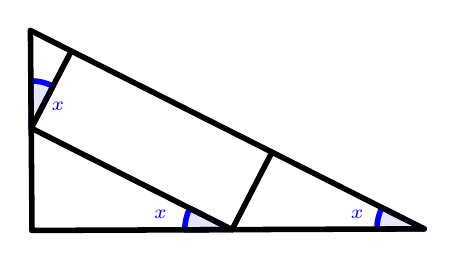
\begin{tikzpicture}[line cap=round,line join=round,>=triangle 45,x=1cm,y=1cm]
\draw [shift={(-2.35,-1.53)},line width=2pt,color=blue,fill=blue,fill opacity=0.10000000149011612] (0,0) -- (153.25189583707856:0.6) arc (153.25189583707856:180.23010229509723:0.6) -- cycle;
\draw [shift={(-4.790201606399793,-1.5398000064514048)},line width=2pt,color=blue,fill=blue,fill opacity=0.10000000149011612] (0,0) -- (153.17128410027803:0.6) arc (153.17128410027803:180.23010229509723:0.6) -- cycle;
\draw [shift={(-7.340235585864848,-0.25008059516429015)},line width=2pt,color=blue,fill=blue,fill opacity=0.10000000149011612] (0,0) -- (62.504407536288795:0.6) arc (62.504407536288795:90.45113854678726:0.6) -- cycle;
\draw [line width=2pt] (-7.33,-1.55)-- (-2.35,-1.53);
\draw [line width=2pt] (-7.35,0.99)-- (-2.35,-1.53);
\draw [line width=2pt] (-7.35,0.99)-- (-7.33,-1.55);
\draw [line width=2pt] (-4.790201606399793,-1.5398000064514048)-- (-7.340235585864848,-0.25008059516429015);
\draw [line width=2pt] (-7.340235585864848,-0.25008059516429015)-- (-6.830963560273553,0.7284056343778706);
\draw [line width=2pt] (-4.790201606399793,-1.5398000064514048)-- (-4.282862100643054,-0.5558375012759007);
\begin{scriptsize}
\draw[color=blue] (-3.2,-1.35) node {$x$};
\draw[color=blue] (-5.7,-1.35) node {$x$};
\draw[color=blue] (-7,0.02) node {$x$};
\end{scriptsize}

        \end{tikzpicture}
        \end{turn}
    \end{figure}
    First, note by AAA criteria that all three similar triangles are similar to the large right triangle. Let the length of the box as  $l$ and the width as $w$. ($l$ denotes the segment that coincides with the long hypotanuse). Then, $5 = l+\frac{3w}{4}+\frac{4w}{3} = l +\frac{25w}{12}$ by similarity. Hence, $l = 5-\frac{25w}{12}$. We want to maximize $lw$, which is equal to $w(5-\frac{25w}{12}) = -\frac{25}{12}w^2+5w = -\frac{1}{12}(5w-6)^2+3$. Hence, the maximum area is 3, which is achieved by $w = \frac{6}{5}$ and $l = \frac{3}{\frac{6}{5}} = \frac{5}{2}$.
    
    \section*{Problem 5}
    \begin{enumerate}[a.]
        \item By arc length formula, the length is $$\int_0 ^{\frac{\pi}{4}} \sqrt{1+\left(\frac{d}{dx} \int _0 ^x \sqrt{\cos{2t}} dt\right)^2} = \int_0 ^{\frac{\pi}{4}} \sqrt{1+\cos 2x} dx = \int_0 ^{\frac{\pi}{4}} \sqrt{2} \cos{x} dx = 1.$$
        \item \begin{enumerate} [i.]
        % Different qn but cool vid: https://www.youtube.com/watch?v=QCAax866If4
            \item We will prove that $\lim_{x \rightarrow 0^{+}}x\ln{x} = f(0)$. By L-hopital's rule, $$\lim_{x \rightarrow 0^{+}}x\ln{x} = \lim_{x \rightarrow 0^{+}} \frac{\ln{x}}{\frac{1}{x}} = \lim_{x \rightarrow 0^{+}} \frac{\frac{1}{x}}{-\frac{1}{x^2}} = \lim_{x \rightarrow 0^{+}} -x = 0 = f(0).$$
            
            Hence, $f$ is continuous at 0  from the right.
            
            \item Since $f$ is continuous from the right, we just add like normal. By chain rule, one can verify that  $\int x^2 \ln{x}^2 = \frac{x^3}{27} (9 \ln{x}^2-6\ln{x}+2) + C$. The volume is
            
            % Do we need to split the integrals? I think int^2_0 (xlnx)^2 will work as well right %technically we need to mod out. I am not sure because xlnx is not defined in 0
            \begin{align*}
            V &= \pi \left\lvert \int_0 ^1 (x \ln{x})^2 \right\rvert + \pi \left\lvert \int_1 ^2 (x \ln{x})^2  \right\rvert \\
            &= \pi \left\lvert \frac{x^3}{27} (9 \ln{x}^2-6\ln{x}+2)  \right \rvert_0 ^1 + \pi \left\lvert \frac{x^3}{27} (9 \ln{x}^2-6\ln{x}+2)  \right \rvert_1 ^2 \\
            &= \frac{2}{27}\pi+ \frac{2}{27}(7+36\ln{2}^2-24\ln{2}).
            \end{align*}
        \end{enumerate}
    \end{enumerate}
    \section*{Problem 6}
    \begin{enumerate}[a.]
        \item Note that 
        \begin{align*}
        \lim_{n \rightarrow \infty} \sum_{k=1} ^n \ln{\sqrt[n]{1+\frac{k}{n}}} &= \lim_{n \rightarrow \infty} \frac{1}{n} \sum_{k=1} ^n \ln{\left(1+\frac{k}{n}\right)} \\
        &= \int_0 ^1 \ln{(1+x)} dx \\
        &= \left \lvert  (x+1) \ln{(x+1)} - (x+1) \right \rvert_0 ^1 \\
        &= 2\ln{2}-1. 
        \end{align*}
        (Recall that $\int \ln{x} = x\ln{x}-x+C$ by chain rule).
        \item We prove a lemma.
        \begin{lemma}
        For all positive integer $m$, $$\frac{1}{x(x+1)\cdots(x+m)} = \frac{1}{m!} \left( \sum_{i=0} ^m \binom{m}{i} \frac{1}{x+i} (-1)^i \right). $$
        \end{lemma}
        \begin{proof}
        We use induction on $m$. For $m=1$, the identity is obvious. Assume for $m = k-1$, the identity is correct. Then,
        % In your identity, you have 1/x+i as a factor, but you end up with (1/x+i)^2? I think I have another proof. Mind if I write it out? okay fine. btw where is the 1/(x+i)^2 ?
        
        \begin{align*}
        \frac{1}{x\cdots(x+k)} &= \frac{1}{k} \left( \frac{1}{x\cdots(x+k-1)} - \frac{1}{(x+1)\cdots(x+k)} \right) \\
        &= \frac{1}{k!} \left( \left( \sum_{i=0} ^{k-1} \binom{k-1}{i} \frac{1}{x+i} (-1)^i \right) -\left( \sum_{i=0} ^{k-1} \binom{k-1}{i} \frac{1}{x+i+1} (-1)^i \right) \right)  \\
        &=\frac{1}{k!} \left( \left( \sum_{i=0} ^{k-1} \binom{k-1}{i} \frac{1}{x+i} (-1)^i \right) -\left( \sum_{i=1} ^{k} \binom{k-1}{i} \frac{1}{x+i} (-1)^i \right) \right) \\
        &= \frac{1}{k!} \left( \binom{k-1}{0} \frac{1}{x} + \sum_{i=1}^{k-1} \left( \binom{k-1}{i}+\binom{k-1}{i-1} \right) \frac{1}{x+i} (-1)^i +  \binom{k-1}{k} \frac{1}{x+k}(-1)^k  \right)  \\
        &= \frac{1}{k!} \left( \sum_{i=0} ^k \frac{1}{x+i} \binom{k}{i} \frac{1}{x+i} (-1)^i\right).
        \end{align*}
        (Note that here we define $\binom{k-1}{k} = 1$). Also, we use Pascal's identity i.e. $\binom{n}{k} = \binom{n}{k-1}+\binom{n-1}{k-1}$). Hence, our lemma is proven. 
         \end{proof}
         Now, the answer of our problem is simply $$\int \frac{1}{m!} \left( \sum_{i=0} ^m \binom{m}{i} \frac{1}{x+i} (-1)^i \right) = \frac{1}{m!} \left( \sum_{i=0} ^m \binom{m}{i} \ln{|x+i|} (-1)^i \right)+C.$$
         
         
         \begin{proof}
         We want to split the fraction $\frac{1}{x(x+1)...(x+m)}$ into partial fractions. To do this, put,
         \begin{equation*}
             \frac{1}{x(x+1)...(x+m)} = \frac{A_0}{x} + \frac{A_1}{x+1} + \frac{A_2}{x+2} + \cdots + \frac{A_m}{ x+m}.
         \end{equation*}
         Multiplying the denominator out, we get,
         \begin{equation*}
             [A_0(x+1)...(x+m)] + [A_1(x)...(x+m)] + \cdots + [A_m(x)...(x+m-1)] = 1
         \end{equation*}
         For each $A_i$, it is multiplied by $(x)(x+1)...(x+i-1)(x+i+1)...(x+m)$. Subbing in $x=-i$ removes all terms and leaves
         \begin{equation*}
             A_i(-i)(-i+1)...(-i+i-1)(-i+i+1)...(-i+m)=1 \implies A_i (-1)^i i!(m-i)! = 1.
         \end{equation*}
         Hence, the term $A_i$ in the partial fraction expansion must be,
         \begin{equation*}
             A_i = (-1)^i \frac{1}{i!(m-i)!} = (-1)^i \frac{1}{m!} \binom{m}{i}
         \end{equation*}
         When the integral acts on each $\frac{A_i}{x+i}$ term, we have,
         \begin{equation*}
             \int \frac{A_i}{x+i} = (-1)^i \frac{1}{m!} \binom{m}{i} \ln|x+i|
         \end{equation*}
         Hence, 
         \begin{equation*}
             \int \frac{A_0}{x} + \frac{A_1}{x+1} + \frac{A_2}{x+2} + \cdots + \frac{A_m}{x+m} = \sum_{i=0}^m \left[(-1)^i \frac{1}{m!} \binom{m}{i} \ln|x+i|\right] + C
         \end{equation*}
         \end{proof}
       
    \end{enumerate}
    \section*{Problem 7}
    % Oh I like this way of solving the problem. Seems very clean
    \begin{enumerate}[a.]
        \item 
        \begin{align*}
            \frac{dy}{dx}+\frac{y}{e^y+x} &= 0\\
            e^ydy+xdy+ydx &= 0\\
            xdy+ydx &= -e^ydy \\
            (xy)' &= -e^ydy \\
            xy &= \int -e^y dy\\
            xy &= -e^y+C
        \end{align*}
        Since $y(0) = 1$, we see that $C=e$. Hence, the solution is $xy+e^y=e$.
    \item 
    \begin{enumerate}[i.] %i suck at diff eqns please check
    % changed the height of the black cone to k so it's less confusing
        \item Let $k$ be the height of the "grey cone" and $v$ be the volume at a given time. So $h=16-k$. Then, $\frac{dk}{dt} = \frac{\sqrt{k}}{2}$, which means $\frac{2}{\sqrt{k}}dk = dt$. Hence, $t = 4\sqrt{k}+C$. At $t=0$, $k=0$. Hence, $C=0$. Thus, $t = 4\sqrt{k}$. Finally, the height of the water is $h = 16 - 4\sqrt{t}$. 

        \item When $h=0$, $4\sqrt{t} = 16$, hence  $t=16$.
    \end{enumerate}
    
    \end{enumerate}
    \section*{Problem 8}
    \subsection*{Proof 1}
    Let $F(x) = \int_0 ^x f(x) dx$. Since it converges, it has a limit $L$ as $x \to \infty$. Assume by contradiction that $xf(x)$ does not converge to 0. Then there exists $c>0$ so that $xf(x)>0$ for arbitary large $x$.  Suppose $x_0f(x_0)>c$ for $x_0$ large enough and $\int_{x_0} ^\infty f(t)dt < d$. Pick $x_1>2x_0$ such that $x_1f(x_1) > c$. Since $f$ is monotone decreasing, $\int_{x_0} ^{x_1} f(x) dx > (x_1-x_0)f(x_1) > (x_1-x_0)\frac{c}{x_1}  = c\left(1-\frac{x_0}{x_1}\right)>\frac{c}{2} $. Hence, $d > \int_{x_0} ^\infty f(t)dt > \frac{c}{2}$. Since $\lim_{x \rightarrow \infty} \int_x ^\infty f(t)dt = 0$, we can pick $x_0$ large enough so that $d$ is smaller than $\frac{c}{2}$, contradiction. Hence, the limit is 0.
    \subsection*{Proof 2} Set $F(x) = \int_0 ^x f(x) dx$. Since $F(x) \to L$, for $\epsilon/4$ there exists some $N>0$ such that whenever $x>N$, $F(x) \in (L+\epsilon/4, L-\epsilon/4)$. Pick any $n,m >N$, and we have $F(n) \in (L+\epsilon/4, L-\epsilon/4)$ and $F(m) \in (L+\epsilon/4, L-\epsilon/4)$. This means that whenever $n,m >N$\footnote{This is a theorem in analysis saying that convergent sequences are Cauchy.},
    \begin{equation}
        -\epsilon/2<\int^n_m f(x) dx<\epsilon/2. \label{eq1} 
    \end{equation}
    Now, either there is some point $x_0$ which $f$ touches the $x$-axis or not. If there isn't, since $f$ is decreasing, $f$ lies entirely above the $x$-axis. Fix $k \in \mathbb{R}$ such that $k>N$. Then $2k>N$ and from (\ref{eq1}),
    \begin{equation*}
        -\epsilon/2<\int^{2k}_k f(x) dx < \epsilon/2 \implies 0<\int^{2k}_k f(x) dx < \epsilon/2.
    \end{equation*}
    However, since $f$ is decreasing, 
    \begin{equation*}
        0< kf(2k) \leq \int^{2k}_k f(x) dx < \epsilon/2 \implies 2kf(2k)<\epsilon
    \end{equation*}
    (Here, $kf(2k)$ is derived from $\int^{2k}_k f(2k) dx \leq \int^{2k}_k f(x) dx$). So for any $x>2k$, $0<xf(x)<\epsilon$, implying that $xf(x)$ converges to 0. \\
    
    Else, suppose there is some point $x_0$ where the $f$ touches the $x$-axis. Put $M=\max\{x_0, N\}$. Since $f$ is decreasing, whenever $x>M$, $f(x) \leq 0$. Again, fix $k \in \mathbb{R}$ such that $k>M$, then $2k>M$. From (\ref{eq1}),
    \begin{equation*}
        -\epsilon/2<\int^{2k}_k f(x) < \epsilon/2 \implies -\epsilon/2<\int^{2k}_k f(x) \leq 0.
    \end{equation*}
    Again, since $f$ is decreasing, 
    \begin{equation*}
        -\epsilon/2 < \int^{2k}_k f(x) \leq kf(2k) \leq 0 \implies -\epsilon < 2kf(2k)\leq 0
    \end{equation*}
    Whenever $x>2k$, $-\epsilon<xf(x)<0$. For all $\epsilon$, there exists some $N \in \mathbb{R}$ such that $n>N$ implies $|nf(n)|<\epsilon$, $xf(x)$ must converge to $0$ as $x \to \infty$. 
\end{document}